%%%%%%%%%%%%%%%%%%%%%%%%%%%%%%%%%%%%%%%%%%%%%%%%%%%%%%%%%%%%%%%%%%%%%%%%%%%%%%%
%% Active Learning Machine Learning Methodology and Results
%%
%%
%% Points to mention:
%%    Voronoi is used because it is insensitive to volume expansions of structure
%%    TODO: Explain PCA analysis
%%    TODO: Get PCA reference
%%
%% TODO:
%%    Why AB2 and AB3
%%    TEMP
%%%%%%%%%%%%%%%%%%%%%%%%%%%%%%%%%%%%%%%%%%%%%%%%%%%%%%%%%%%%%%%%%%%%%%%%%%%%%%%


% ################################# Paragraph #################################
% %%%%%%%%%%%%%%%%%%%%%%%%%%%%%%%%%%%%%%%%%%%%%%%%%%%%%%%%%%%%%%%%%%%%%%%%%%%%%
% General intro to AL scheme
% Basic gist, i.e. define our candidate space of materials to explore within
% (we do this by looking taking all structurally unique systems in DBs)
% To start the AL we take the few systems that have DFT calcs (more generally
% we can just choose random structures)
% We then build a surrogate model (GP, initially really bad) to predict the
% stability of the entire candidate space
% %%%%%%%%%%%%%%%%%%%%%%%%%%%%%%%%%%%%%%%%%%%%%%%%%%%%%%%%%%%%%%%%%%%%%%%%%%%%%
% | - Paragraph start

Here, we present a machine-learning based methodology for discovering new stable and meta-stable phases of Iridium oxide. 

Our approach builds on the principles of surrogate active learning, where a model is iteratively trained on available ab-initio DFT data. The model predictions are used as a surrogate to the DFT energy evaluations, which are used to acquire new systems for DFT in the population based on an acquisition criteria.
%
Machine learning accelerated active learning procedures have been demonstrated to successfully speed up materials discovery in conjugation with genetic algorithms for alloy nanoparticles \cite{Jennings2019, EXAMPLE_1, and EXAMPLE_2}.
% TEMP
The methodology consists of two steps, the first being the generation of the candidate space,
which is an inclusive list of all initial crystal structures to be screened through during the search routine. Since the initial candidates sets a formal limit for the structures that can ultimately be discovered, it is crucial to define a candidate space that is sufficiently broad and diverse, if anything novel is to be found.

%Here it is crucial to ensure that the candidate 
%
%This part is really important because you can't discover anything interesting if it's not a part of the candidate space to begin with.
% TEMP Say more
The second part of the algorithm is iterative active learning algorithm.
% TODO Add figure reference
The procedural flow diagram is shown in figure TEMP.

% | - __old__
% Our machine learning accelerated materials discovery method proceeds through the following steps:
% First, the dataset of candidate materials is constructed.
% This data set will define the totality of materials that will be considered by the search algorithm,
% this is done because the search space of materials is not a continous space but a discrite array of individual structures.
% Next, the dataset of materials is transformed into a vectorial representation by using a fingerprinting method that encodes the relevent chemical and structural information.
% __|

% __|


% ################################# Paragraph #################################
% %%%%%%%%%%%%%%%%%%%%%%%%%%%%%%%%%%%%%%%%%%%%%%%%%%%%%%%%%%%%%%%%%%%%%%%%%%%%%
% Data prep. | Unique Structures | Atom subst., V relax | Fingerprinting
% Probably most of this needs to go to SI
% %%%%%%%%%%%%%%%%%%%%%%%%%%%%%%%%%%%%%%%%%%%%%%%%%%%%%%%%%%%%%%%%%%%%%%%%%%%%%
% | - Paragraph start
The structures that comprise the candidate data set were constructed by parsing for structurally unique systems in the OQMD and Materials Project DFT databases.
%
The structural uniqueness was performed using a space-group symmetry classification scheme developed by Jain et al. \cite{Jain2018},
which can classify a structure based on its composition and structure.
 (see SI for more details on the structural classification scheme).
%
This structural classification scheme can directly serve as a structural fingerprint and has successfully been applied towards the prediction of formation energies of inorganic compounds \cite{Jain2018}
%
To focus the scope of the study, only \ABtwo  and \ABthree stoichiometries were parsed from the databases.
%
The \ABtwo formula was chosen because it includes \rIrOtwo, the known most stable polymorph of \IrOtwo.
%
Importantly, \ABthree was chosen to include high valency \IrOthree structures in our search.
%
The results of the classification scheme resulted in a XYZ AB2 and XYZ AB3 structural prototypes for which iridium and oxygen were replaced for A and B sites, respectively.
%
Finally, a coarse isotropic volume relaxation based on atomic radii was performed on the structures to accommodate the atomic radii of iridium and oxygen into the lattice.
%
Finally, a Voronoi tessellation based fingerprinting scheme developed by Ward et al. \cite{Ward2017} was used to encode the relevant chemical information for each structure into a vector quantity of length 271.
%
The Voronoi based method was used because it is insensitive to volume relaxation.
%
Separate, independent models were used for IrO2 and IrO3 to reduce the complexity of the space, this has the additional effect of making a large number of the fingerprint descriptors redundant.
% How many columns of the 271 are redundant if stoich and composition are frozen
As a result, the 271 length feature space is reduced to a TEMP length vector.
%
PCA was used to reduce the dimensionality of the feature space from 271 to 20 features such that 99 \% of the variance is captured \cite{Tipping1999}.
% __|


% ################################# Paragraph #################################
% %%%%%%%%%%%%%%%%%%%%%%%%%%%%%%%%%%%%%%%%%%%%%%%%%%%%%%%%%%%%%%%%%%%%%%%%%%%%%
% Iterative Training of Gaussian Process
% TODO go through fingerprinting here, not previous part
% %%%%%%%%%%%%%%%%%%%%%%%%%%%%%%%%%%%%%%%%%%%%%%%%%%%%%%%%%%%%%%%%%%%%%%%%%%%%%
% | - Paragraph start
The active learning algorithm proceeds through iterative ML training, prediction, and acquisition steps and is visualized in figure TEMP.
%
While any regression technique can be used, we employed the Gaussian process (GP) regression model because it offers a high degree of flexibility and, most importantly, built-in uncertainty quantification.
% TODO: Does the acquisition function we use have a name?
Uncertainty quantification on the predicted formation energies is important because its used in the acquisition criteria.
%
Further details on the GP model, including hyper parameter information, is including in the SI.
%
The acquisition is made by selecting the $N$ systems with the lowest value of the acquisition function.
%
The acquisition function is defined in terms of the predicted formation energy, E, and the uncertainty, U:

\begin{equation}
    F = E - \kappa U,
\end{equation}

where the parameter $\kappa$ can be tuned to probe low uncertainty (small $\kappa$) or high uncertainty regions  (large $\kappa$).
% TODO: Write aquisition function here, again does it have a name
%$a = b + c$
%
The value of $N$ determines how many structures are selected for DFT calculations,
and as such, determines the degree of parallization of the routine. The optimal value of $N$ depends on the computational resources available, as small values of N result in an algorithm that is slow, as every DFT calculation is performed serially.
% TODO: Is this statement true?
Larger values of N speed up the active-learning algorithm, but leads to a higher number of DFT calculations performed before convergence. %but potentially decreases the efficiency of the algorithm by TEMP TEMP.
%
Here we chose a value $N=10$.
%
The acquired structures are initially volume relaxed, followed by a full relaxation of all of the atomic coordinates,
see SI for additional details on the DFT methodology.
% This is wordy
The AL loop proceeds until convergence is achieved, which here is defined as the point at which %the model has determined the lowest $N$ structures and has achieved a degree of accuracy for the candidate space such that
no structures have predicted formation energies with an uncertainty bound lower than the most stable $N$ structures.
% __|


% | - AL steps itemized
\begin{enumerate}
  \item Candidate space of structures is generated
  \item Initial seed data is used to train a ML model
  \item ML model predicts energy of entire candidate space
  \item Most valuable structure(s) is(are) selected using acquisition function
  \item DFT calculation(s) is(are) performed to obtain additional training data points
  \item ML model is retrained with additional data
  \item Repeat steps (3) through (6) until convergence criteria is reached
  % \item TEMP
\end{enumerate}
% __|


% | - Figure | Active Learning Algorithm **************************************
\begin{figure*}
\centering
\makebox[\textwidth][c]{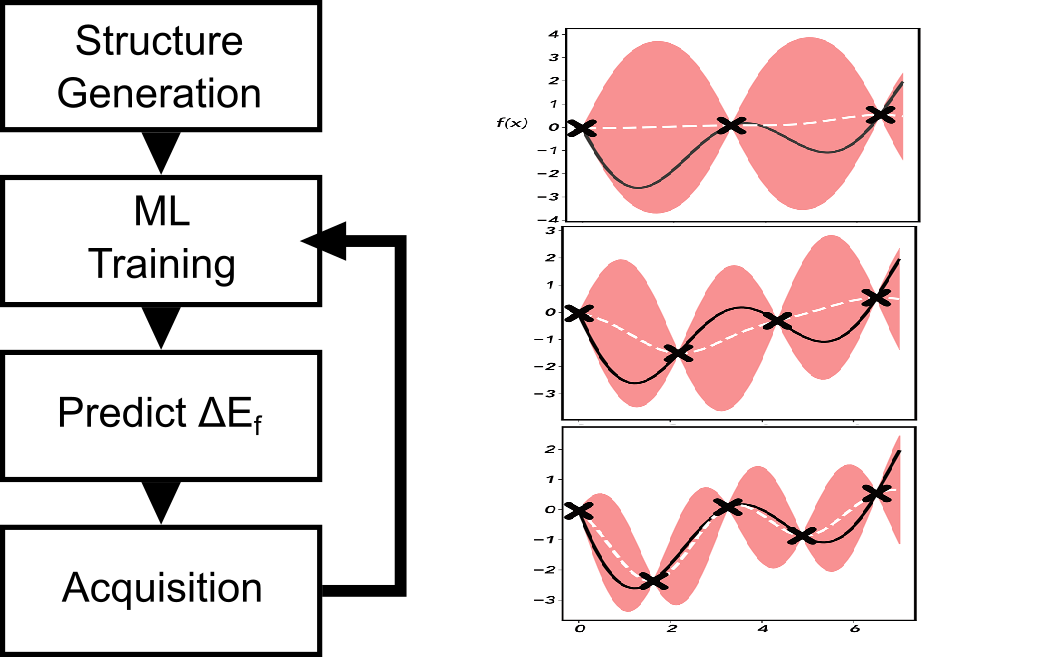
\includegraphics
  {02_figures/Surrogate_model_mine.png}
  }
\caption{\label{fig:all_diagram}
(a) Active learning algorithm diagram.
First the candidate space of structures is generated,
next, the machine learning model is trained on any available DFT formation energy data.
The trained ML model is then used to predict the DE of the entire candidate space.
Finally, an acquisition step is performed to pick the next most valuable calculation to perform an-initio DFT on
% -----------------------------------------------------------------------------
(b) Toy model demonstrating a GP model converging with each subsequent iteration.
% -----------------------------------------------------------------------------
}
\end{figure*}
% __|






% #############################################################################
% #############################################################################
% ██████  ███████ ███████ ██    ██ ██   ████████ ███████
% ██   ██ ██      ██      ██    ██ ██      ██    ██
% ██████  █████   ███████ ██    ██ ██      ██    ███████
% ██   ██ ██           ██ ██    ██ ██      ██         ██
% ██   ██ ███████ ███████  ██████  ███████ ██    ███████
% #############################################################################
% #############################################################################
% Notes:
%   - QUESTION Is there any physical intuition that we can gleam from the fingerprints?
%   - QUESTION What did @Chris mean by this? "Computed amorphous phase to define synthesizability"
% #############################################################################
% #############################################################################



% ################################# Paragraph #################################
% %%%%%%%%%%%%%%%%%%%%%%%%%%%%%%%%%%%%%%%%%%%%%%%%%%%%%%%%%%%%%%%%%%%%%%%%%%%%%
% Intro/transition paragraph
%
% %%%%%%%%%%%%%%%%%%%%%%%%%%%%%%%%%%%%%%%%%%%%%%%%%%%%%%%%%%%%%%%%%%%%%%%%%%%%%
% | - Paragraph start
%
We now turn our attention of the application of this active learning scheme by
applying them to IrO2 and IrO3.
%
The AL algorithm is applied separately to IrO2 and IrO3 because we are specifically interested in the most stable polymorphs at each stoicheometry.
% TODO How many features drop out when you constrain the stoich.?
This has an the added benefit of reducing the number of fingerprint vectors from the Voronoi tesselation dramatically (from TEMP to TEMP) because many features are senstive to changes in stoicheometry.
% __|

% ################################# Paragraph #################################
% %%%%%%%%%%%%%%%%%%%%%%%%%%%%%%%%%%%%%%%%%%%%%%%%%%%%%%%%%%%%%%%%%%%%%%%%%%%%%
% Results for IrO3
% MAIN RESULTS:
%   How many generations to find top 2-3 structures?
% We need to call them something else than "convergence plots" (bad name)
% %%%%%%%%%%%%%%%%%%%%%%%%%%%%%%%%%%%%%%%%%%%%%%%%%%%%%%%%%%%%%%%%%%%%%%%%%%%%%
% | - Paragraph start
%
Figure TEMP a and b shows several plots of the AL predictions on the candidate space at particular generations of the AL algorithm for the IrO3 candidate space with an aquisition bin size of 10 DFT calculations per iteration and an initial 11 calculations used for seeding.
%
Figure TEMP a. shows the progression of the model at select generations of the active learning loop.
%
It can be seen from Figure TEMP a that
%
Figure TEMP b. shows the
The formation energy, either predicted (small colored circles) or computed (large red-bordered circles), is plotted on the y-axis against all structures in the candidate space of IrO3 polymorphs.
%
The DFT derived formation energy is plotted alongside the predicted data (hollow diamonds).
%
It is evident from figure TEMP, that the Gaussian process model is doing a poor job of predicting the DFT formation energy of the candidate space, with a exceptionally poor MAE of TEMP eV/atom at the AL generation shown here.
%
This is significatally lower than the leave-one out cross validation error of TEMP ~0.15 eV/atom, which indicates that the issue does not lie with a poor predictive model.
%
Instead, the issue lies with the large degree of structural reorganization that occurs over the course of a typical DFT ionic optimization.
% TODO Change wording when @Kirsten uses the protosearch to optimize candidates
Becasue the candidate space structures are generated
% To compare the performance of the AL routine we compare against a
% __|


% | - Figure | IrO3 Convergence Plot
\begin{figure*}
\centering
\makebox[\textwidth][c]{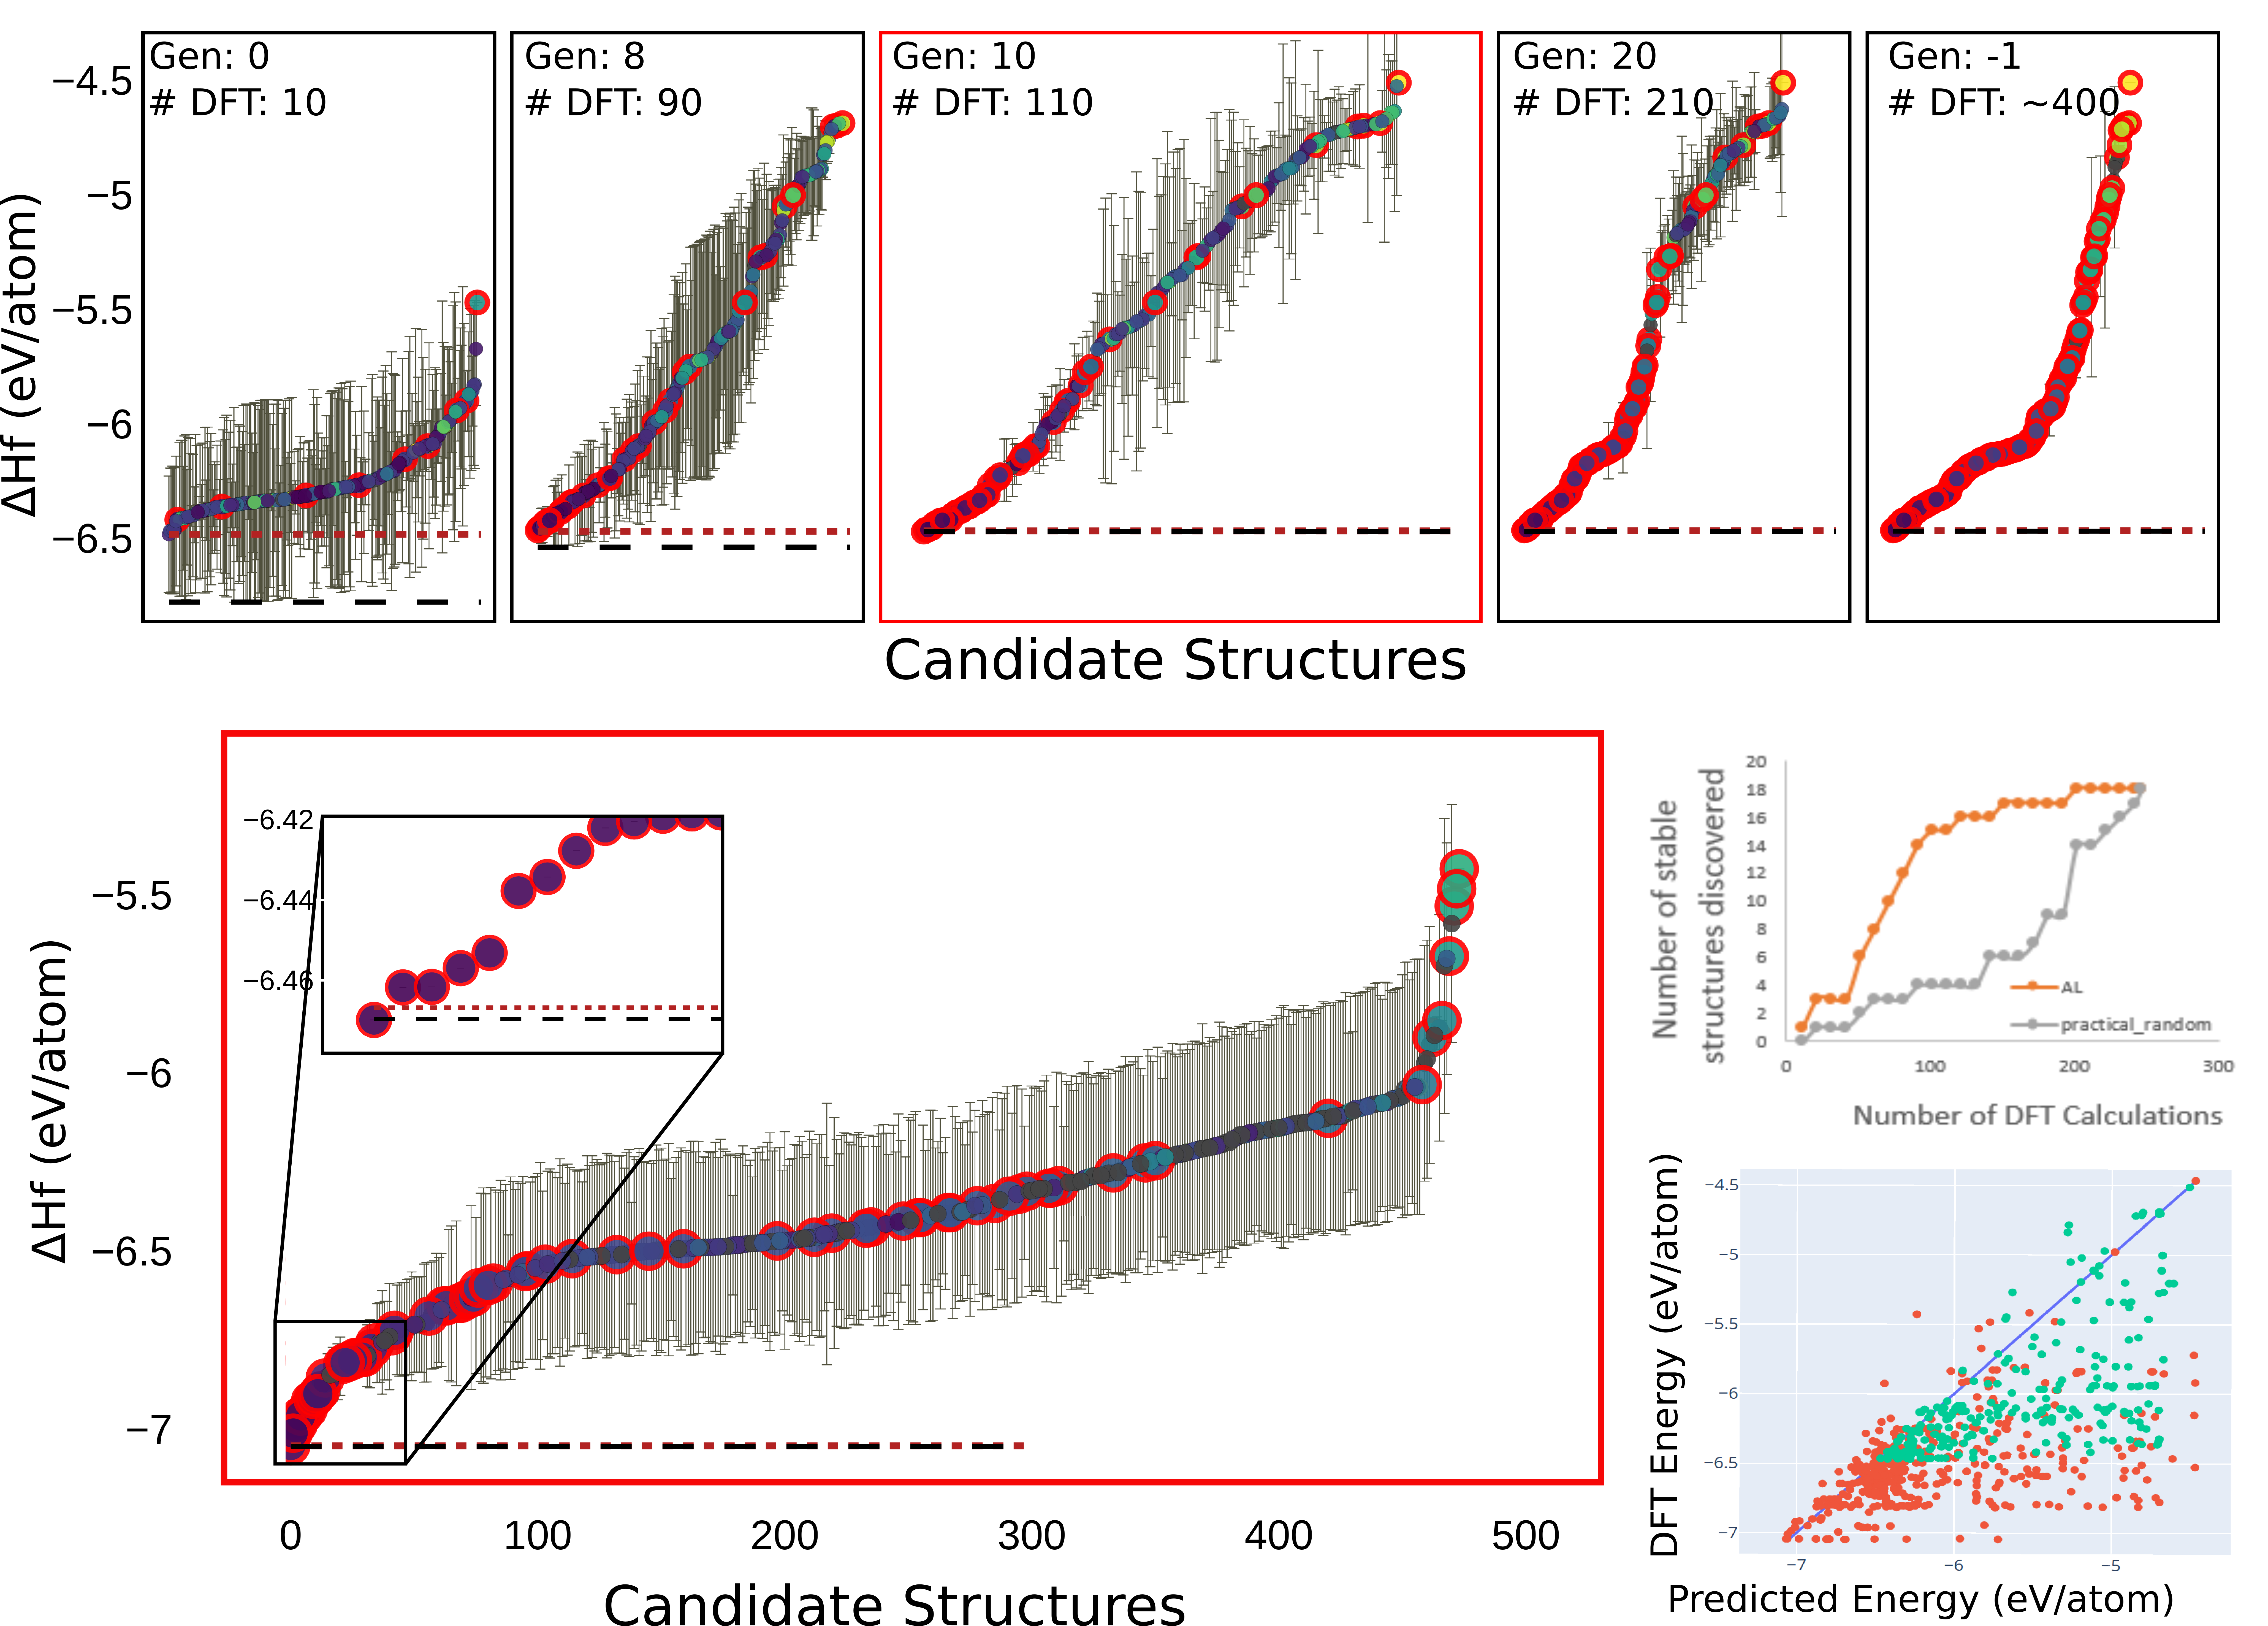
\includegraphics[width=\textwidth,height=\textheight,keepaspectratio]
{02_figures/ml_convergence_plots/test_iro3_al.jpg}
}
\caption{\label{fig:iro2_al}
Results from machine-learning accelarted active learning material discovery algorithm.
% FORMATION ENTHALPY, FIX
Both (a) and (b) plot the formation enthalpy (either predicted from the model or computed by DFT) for each system in the candidate pool, ordered by decreasing stability (low to high formation energy).
%
Formation energies predicted by the surrogate model are represented by smaller circles,
while aquired DFT formation energies are shown as enlarged red bordered circles.
%
Each data point is colored based on the ordering of the DFT formation energies, with low formation energy systems on the dark end of the spectrum and the highest formation energy species colored light.
%
Error bars representing 1 sigma standard deviation from the Gaussian Process model are shown for each prediction.
%
(a) Series of ML convergence plots at different generations of the active learning algorithm.
%
The middle panel indicates the generation which satisifies the AL stop criteria (see text)
%
(b) Expanded ML plot for the generation that satisfies the stop criteria.
%
Black diamonds indicate the actual DFT formation energy for each system.
%
Inset shows the most stable 20 systems that are within the energetic window of meta-stability (indicated by grey band).
%
(c)
Number of the top 20 polymorphs discovered as a function of the AL generation number for the AL loop using the aquisition criteria in equation TEMP and a control run that utilized a random  aquisition method.


% | - __old__
% Gaussian process machine learning models trained initially on (a) publicly available DFT data for IrO2 and (b) all of the acquired DFT calculations from the active learning algorithm.
% See SI for additional panels at intermediate iterations of the active learning algorithm.
% The Gibbs formation energy (either DFT derived or predicted from the GP model) and associated GP estimated error (2 sigmas or something TEMP) is plotted for each polymorph in the IrO2 candidate space.
% The data points in each subset are ordered from most to least stable (lowest to largest DE formation).
% The individual markers are colored based on their ordering in the final converged GP model.
% Acquired structures are identified by their red borders and slightly larger size.
% The insets show the most stable TEMP structures, where several well known crystal structures are labeled.
% __|

}
\end{figure*}
% __|


% #############################################################################
% | - __old__
% ################################# Paragraph #################################
% AB2 Structures Ankit
% - There are XYZ unique AB2 structures (or multiples, e.g. A2B4)
% - Of those we found 697 unique AB2 prototypes (unique SG/Wyckoff combination) in OQMD/MP
% - To generate our test set we substituted Ir for A and O for B, then isotropically expanded cell volume to constrain a minimum Ir-O distance of XYZ
% - Next translated each of the 697 structures to be described by 271 features (invariant to isotropic expansion/compression), then reduced to 30 using PCA, described in methods XYZ
% - To generate initial training data use existing DFT. Not enough on \ce{IrO_2}, so used OQMD to generate initial training data from nearest structures in phase space, described in Methods XYZ. Training set of 30 structures in SI XYZ.
% __|
